\documentclass[sigconf]{acmart}

\usepackage[english]{babel}
\usepackage{blindtext}

% Copyright
\renewcommand\footnotetextcopyrightpermission[1]{} % removes footnote with conference info
\setcopyright{none}
%\setcopyright{acmcopyright}
%\setcopyright{acmlicensed}
%\setcopyright{rightsretained}
%\setcopyright{usgov}
%\setcopyright{usgovmixed}
%\setcopyright{cagov}
%\setcopyright{cagovmixed}

\settopmatter{printacmref=false, printccs=false, printfolios=true}

% DOI
\acmDOI{}

% ISBN
\acmISBN{}

%Conference
%\acmConference[Submitted for review to SIGCOMM]{}
%\acmYear{2018}
%\copyrightyear{}

%% {} with no args suppresses printing of the price
\acmPrice{}


\begin{document}
\title{Reproduction: Measuring the Security Harm of TLS Crypto Shortcuts}

%\titlenote{Produces the permission block, and copyright information}
%\subtitle{Extended Abstract}

\author{Jared Crawford}
% \authornote{Note}
% \orcid{1234-5678-9012}
% \affiliation{%
%   \institution{Affiliation}
%   \streetaddress{Address}
%   \city{City} 
%   \state{State} 
%   \postcode{Zipcode}
% }
\email{jared13@stanford.edu}

% The default list of authors is too long for headers}
\renewcommand{\shortauthors}{X.et al.}

\begin{abstract}
    TLS provides secure communication lines between end users and web servers. However, establishing this communication line requires additional overhead in the form of transport level handshake round trips and computationally expensive cryptographic operations. To reduce this overhead in bursty web traffic, HTTPS supports many mechanisms (such as TLS session tickets and private value reuse in public key exchange) to reuse these secure connection values for a short period of time. These performance optimizations tradeoff with the forward secrecy of user web traffic. In early 2016, a team at the University of Michigan investigated the extent to which the most popular sites were reusing these values in order to make site operators more aware of the risk involved in doing so\cite{Springall:2016:MSH:2987443.2987480}. In this report, I attempt to reproduce these findings by collecting more recent data (May 2018) on TLS cryptography shortcutes.
\end{abstract}

\maketitle

\section{Introduction}

The authors made TLS 1.2 handshakes over a nine week period with the Alexa Top Million sites and studied the reuse of private ephemeral values in TLS session resumption, TLS session tickets, and Diffie Helmann key exchange. In addition, the researchers observed more general trends such as the churn of the top million sites and protocol usage statistics. In this report, I present a reproduction of these results two years after the papers publication. Due to time constraints, the data collected spans a comparatively smaller one week period compared to the original paper.

The key results of this paper which I reproduce are Figures 1-4 in the paper. TLS supports user advertised lifetimes of ephemeral secrets. For example, a client can specify that their session key should be deleted after 1 hour to maintain a higher degree of forward secrecy. Figures 1-2 demonstrate how compliants sites are with these advertised ephemeral lifetimes. Figures 3-4 show how long (in days) that session ticket encryption keys are reused by sites. Reuse of encryption keys expose users to additional risk because it requires that the server save a copy of these keys for their lifetime. Thus, if a malicious party gains server-side access to a site which reuses keys for one week, client communications during the past week can be retroactively decrypted. Additionally, I present a summary of what TLS features are supported by popular domains (e.g. "of the Majestic Million websites that support HTTPS, 83\% support session ID resumption and 76\% support session tickets.") This data for this analyisis was collected over a one week day period from May 26 to June 2.

Churn Figure
\begin{figure}[tp]
\centering
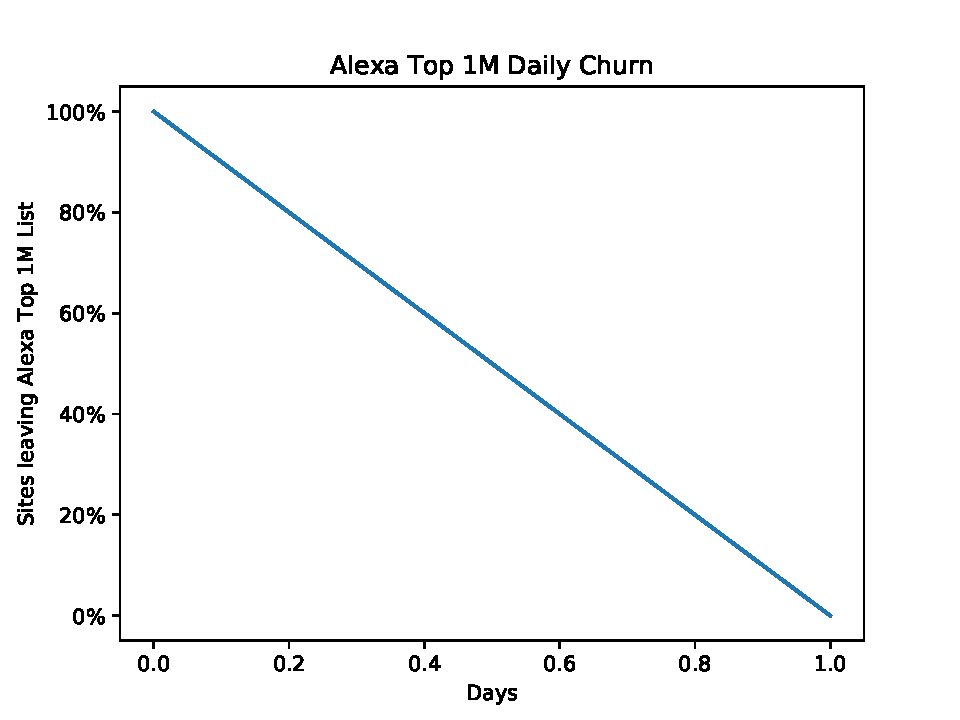
\includegraphics{figures/churn.png}
\caption{\blindtext}
\end{figure}


\section{Reproductions}

\subsection{Figures 1-2}
Figure 1
\begin{figure}[tp]
\centering
\includegraphics{figures/id_minutely_cdf.png}
\caption{\blindtext}
\end{figure}

Figure 2
\begin{figure}[tp]
\centering
\includegraphics{figures/stek_minutely_cdf.png}
\caption{\blindtext}
\end{figure}

\subsection{Figures 3-4}
Figure 3
\begin{figure}[tp]
\centering
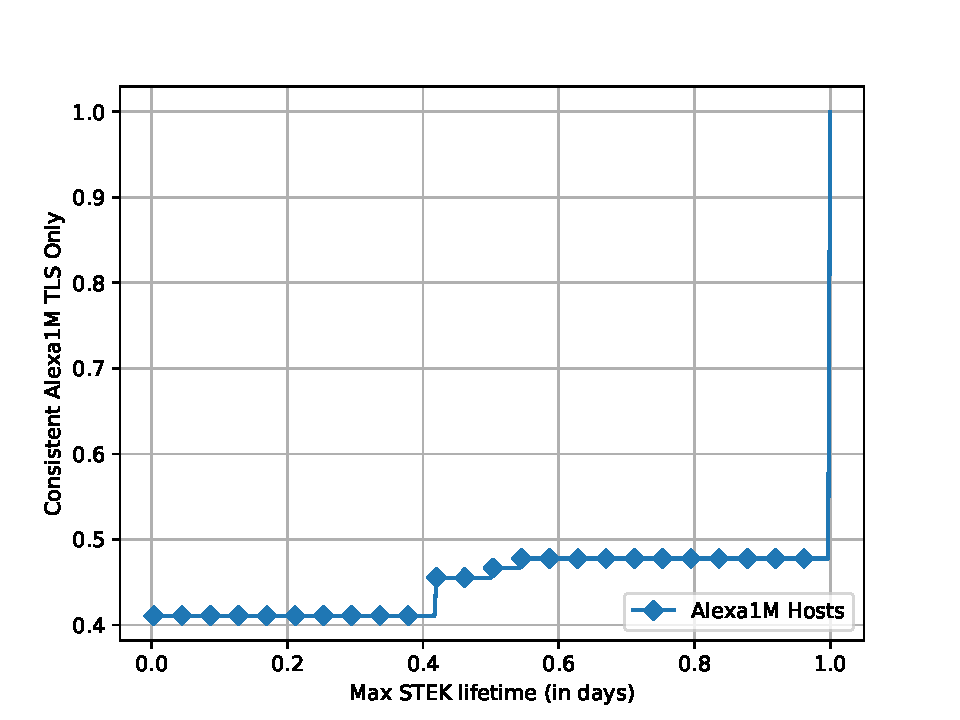
\includegraphics{figures/max_stek_cdf.png}
\caption{\blindtext}
\end{figure}

Figure 4
\begin{figure}[tp]
\centering
\includegraphics{figures/stek_stacked.png}
\caption{\blindtext}
\end{figure}

\section{Evaluation}

\section{Conclusion}

\bibliographystyle{ACM-Reference-Format}
\bibliography{reference}

\end{document}